\section{Auswertung}
\label{sec:Auswertung}

Die Graphen werden sowohl mit Matplotlib \cite{matplotlib} als auch NumPy \cite{numpy} erstellt. Die Fehlerrechnung wird mithilfe von Uncertainties \cite{uncertainties} durchgeführt. Für Konstanten wird SciPy \cite{scipy} verwendet.

\subsection{Bestimmung des vertikalen Erdmagnetfelds}

Das vertikale Magnetfeld wird durch ein vertikales Helmholtzspulenpaar kompensiert. Es kann also bei einem angelegten Strom von $\SI{229}{\milli\ampere}$ und Formel \eqref{eq:helmholtz} bestimmt werden zu:
\[
B_.{Erde,v} \approx \SI{35.1}{\micro\tesla}
\]
Die die Helmholtzspule besitzt dabei den Radius $R=\SI{11,735}{\centi\metre}$ und eine Windungszahl von $N=20$ \cite{V21}.

\subsection{Bestimmung des horizontalen Erdmagnetfelds und der Kernspins}

Es wird in Abhängigkeit der Modulationsfrequenz $\nu$ das benötigte horizontale B-Feld für die Resonanzen der beiden Rb-Isotope vermessen. Das gesamte B-Feld setzt sich zusammen aus dem der Sweep- und der Horizontalfeld-Spule. Die gemessenen Werte, sowie die nach Formel \ref{eq:helmholtz} berechneten Werte der B-Felder sind in Tabelle \ref{tab:messung1} eingetragen. Hier sind die Werte für die Sweep-Spule gegeben als $R=\SI{16.39}{\centi\metre}$ und $N=11$, sowie für die Horizontalfeld-Spule $R=\SI{15.79}{\centi\metre}$ und $N=154$ \cite{V21}.
Es wird das gesamte horizontale B-Feld $B_.{Ges,i}$ der beiden Rb-Isotope gegen $\nu$ aufgetragen und eine lineare Ausgleichsrechnung der Form
\[
B_.{Ges,i}(\nu) = a_i\nu + b_i
\]
durchgeführt (vergleiche Abbildung \ref{fig:messung1}).
Es ergeben sich die Parameter:
\begin{align*}
a_1 &= \SI{1.475(17)e-10}{\tesla\per\hertz}\\
a_2 &= \SI{2.185(12)e-10}{\tesla\per\hertz}\\
b_1 &= \SI{14.3(11)}{\micro\tesla}\\
b_2 &= \SI{15.3(8)}{\micro\tesla}\text{.}\\
\end{align*}
Der Parameter $b$ entspricht hier dem horizontalen Erdmagnetfeld. Gemittelt ergibt sich so:
\[
B_.{Erde,h} = \SI{14.8(5)}{\micro\tesla}\text{.}
\]
Der Fehler ist hier der Fehler auf den Mittelwert.
Die Landé-Faktoren sind mit dem Parameter $a$ mithilfe von Gleichung \eqref{eqn:B_M_Theorie} verknüpft über
\begin{equation*}
g_{F,i}=\frac{4\pi m_e}{e a_i} \text{.}
\end{equation*}
Damit ergeben sich die Werte
\begin{align*}
g_{F,1} &= \num{0.484(6)}\\
g_{F,2} &= \num{0.327(18)}\text{.}
\end{align*}
Der Kernspin wird mit Formel \eqref{eqn:g_F_Theorie} berechnet. Dabei ist $L=0$, $S=0,5$, $J=0,5$ und $g_J$ ergibt sich mit Formel \eqref{eqn:g_J_Theorie} zu $g_J=2,0023$. 
Somit ergeben sich die Werte:
\begin{align*}
I_.A &= \num{1.567(24)}\\
I_.B &= \num{2.561(17)}
\end{align*}
Die Fehler stammen aus der Gaußschen Fehlerfortpflanzung.
\begin{figure}
	\centering
	\includegraphics[width=\linewidth-60pt,height=\textheight-60pt,keepaspectratio]{build/messung1.pdf}
	\caption{Das gesamte horizontale B-Feld $B_.{Ges,i}$ aufgetragen gegen die Modulationsfrequenz $\nu$ für die beiden Rb-Isotope A und B.}
	\label{fig:messung1}
\end{figure}

\begin{table}
	\centering
	\caption{Messwerte der Ströme $I$ der Sweep(S)-Spule und Horizontalfeld(H)-Spule, sowie die daraus berechneten Magnetfelder $B$ für die beiden Rb-Isotope A und B.}
	\label{tab:messung1A}
	\sisetup{table-format=1.2}
	\begin{tabular}{S[table-format=4.0]S[table-format=3.0]S[table-format=3.0]S[table-format=3.2]S[table-format=3.2]S[table-format=3.2]}
		\toprule
		{$\nu/\si{\kilo\hertz}$} & {$I_\text{S,A}/\si{\milli\ampere}$} & {$I_\text{H,A}/\si{\milli\ampere}$} & {$B_\text{S,A}/\si{\micro\tesla}$} & {$B_\text{H,A}/\si{\micro\tesla}$} & {$B_\text{Ges,A}/\si{\micro\tesla}$} \\
		\midrule
		 100 & 483 &   0 & 29.15 & 0.00 & 29.15 \\
		 200 & 718 &   0 & 43.33 & 0.00 & 43.33 \\
		 300 & 382 &  42 & 23.05 & 36.83 & 59.89 \\
		 400 & 112 &  72 & 6.76 & 63.14 & 69.90 \\
		 500 & 271 &  84 & 16.35 & 73.67 & 90.02 \\
		 600 & 237 & 102 & 14.30 & 89.45 & 103.75 \\
		 700 & 129 & 126 & 7.78 & 110.50 & 118.28 \\
		 800 & 368 & 126 & 22.21 & 110.50 & 132.71 \\
		 900 &  69 & 162 & 4.16 & 142.07 & 146.23 \\
		1000 & 582 & 144 & 35.12 & 126.28 & 161.41 \\
		\bottomrule
	\end{tabular}

	\label{tab:messung1B}
	\sisetup{table-format=1.2}
	\begin{tabular}{S[table-format=4.0]S[table-format=3.0]S[table-format=3.0]S[table-format=3.2]S[table-format=3.2]S[table-format=3.2]}
		\toprule
		{$\nu/\si{\kilo\hertz}$} & {$I_\text{S,B}/\si{\milli\ampere}$} & {$I_\text{H,B}/\si{\milli\ampere}$} & {$B_\text{S,B}/\si{\micro\tesla}$} & {$B_\text{H,B}/\si{\micro\tesla}$} & {$B_\text{Ges,B}/\si{\micro\tesla}$} \\
		\midrule
		 100 & 601 &   0 & 36.27 & 0.00 & 36.27 \\
		 200 & 952 &   0 & 57.45 & 0.00 & 57.45 \\
		 300 & 736 &  42 & 44.42 & 36.83 & 81.25 \\
		 400 & 688 &  72 & 41.52 & 63.14 & 104.66 \\
		 500 & 863 &  84 & 52.08 & 73.67 & 125.75 \\
		 600 & 945 & 102 & 57.03 & 89.45 & 146.48 \\
		 700 & 955 & 126 & 57.63 & 110.50 & 168.13 \\
		 800 & 781 & 162 & 47.13 & 142.07 & 189.20 \\
		 900 & 720 & 192 & 43.45 & 168.38 & 211.83 \\
		1000 & 640 & 222 & 38.62 & 194.69 & 233.31 \\
		\bottomrule
	\end{tabular}

	\label{tab:messung1}
\end{table}

\subsection{Bestimmung des Isotopenverhältnisses}

Das Isotopenverhältnis $\xi$ wird aus dem Verhältnis der Tiefe der Resonanzen der Rb-Isotope bestimmt, da diese Proportional zur Menge der Isotope in der Probe ist. In Abbildung \ref{fig:typisch} ist ein typischer Verlauf der Transparenzkurve der Probe bei $\nu=\SI{100}{\kilo\hertz}$ dargestellt.
Das Verhältnis der Resonanztiefen ist gegeben als:
\[
\xi_.{exp} = \frac{\SI{43}{.{px}}}{\SI{19}{.{px}}} \approx 2,263 \text{.}
\]
Das in der Natur vorkommende Verhältnis ergibt sich zu:
\[
\xi_.{theo} = \frac{\text{Anteil}~ \ce{^{85}Rb}}{\text{Anteil}~ \ce{^{87}Rb}}=\frac{\SI{72,17}{\%}}{\SI{27,83}{\%}} \approx 2,593 \text{.}
\]
\begin{figure}
	\centering
	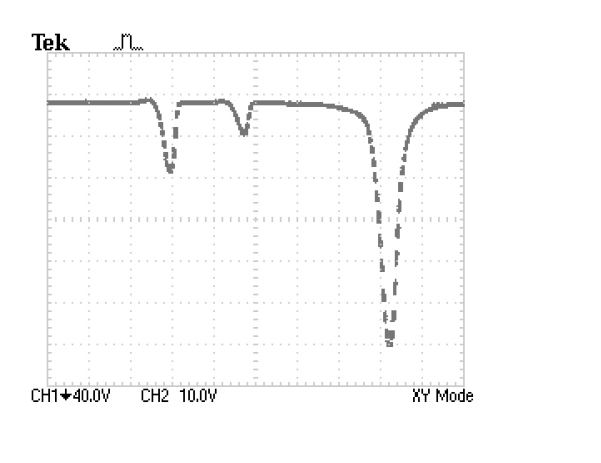
\includegraphics[width=\linewidth-60pt,height=\textheight-60pt,keepaspectratio]{content/images/TEK0006.pdf}
	\caption{Transparenz der Probe in Abhängigkeit des Magnetfeldes bei $\nu=\SI{100}{\kilo\hertz}$. Das B-Feld ist nach links ansteigend.}
	\label{fig:typisch}
\end{figure}

\newpage
\subsection{Abschätzung des quadratischen Zeeman-Effekts}

Die Energieaufspaltung durch den quadratischen Zeeman-Effekt kann durch Formel \eqref{eqn:zeemanDifferenzQuadratisch} dargestellt werden. Die Hyperfeinstrukturaufspaltung der Isotope $\ce{^{85}Rb}$ und $\ce{^{87}Rb}$ des Grundzustandes beträgt \cite{V21}:
\begin{align*}
\Delta E_{85} &= \SI{2.01e-24}{\joule},\\
\Delta E_{87} &= \SI{4.53e-24}{\joule}\text{.}
\end{align*}
Es wird für die Abschätzung das Magnetfeld bei $\nu=\SI{1000}{\kilo\hertz}$ verwendet und $M_F=1$ gesetzt. Einsetzen der $g_{F,i}$ und $B_{.{Ges},i}$ in die Gleichung liefert für den gesamten Zeeman-Effekt:
\begin{align*}
\Delta E_{.{Ges},85} &= \SI{7.25(9)e-28}{\joule}\\
\Delta E_{.{Ges},87} &= \SI{7.07(4)e-28}{\joule},
\end{align*}
wobei der quadratische Term einen Beitrag von
\begin{align*}
\Delta E_{.{quadratisch},85} &= \SI{-1.161(27)e-31}{\joule}\\
\Delta E_{.{quadratisch},87} &= \SI{-2.491(28)e-31}{\joule}
\end{align*}
liefert. Die Fehler stammen aus der Gaußschen Fehlerfortpflanzung.

\subsection{Untersuchung der ansteigenden Flanken der Resonanzen}

Es wird die ansteigende Flanke der Resonanzen in Abhängigkeit der Zeit $t$ untersucht. Dazu wird eine Ausgleichsrechnung der Form
\[
f(t)=1-\exp(-a(t-b))
\]
durchgeführt. Es werden die vom Oszilloskop gespeicherten Daten verwendet. Diese werden auf den Sättigungsbereich normiert.
Es ergeben sich für die Resonanzen der Isotope die Parameter:
\begin{align*}
a_1 &= \SI{0.1201(4)}{\per\milli\second}\\
b_1 &= \SI{-0.535(18)}{\milli\second}\\
a_2 &= \SI{0.1531(10)}{\per\milli\second}\\
b_2 &= \SI{-0.35(4)}{\milli\second}\\
\end{align*}
Die Messwerte und die Ausgleichskurven sind in den Abbildungen \ref{fig:messung2a} und \ref{fig:messung2b} dargestellt. 

\begin{figure}
	\centering
	\includegraphics[width=\linewidth-60pt,height=\textheight-60pt,keepaspectratio]{build/image0.pdf}
	\caption{Transparenz der Probe in Abhängigkeit der Zeit $t$ für die erste Resonanz.}
	\label{fig:messung2a}
\end{figure}

\begin{figure}
	\centering
	\includegraphics[width=\linewidth-60pt,height=\textheight-60pt,keepaspectratio]{build/image2.pdf}
	\caption{Transparenz der Probe in Abhängigkeit der Zeit $t$ für die zweite Resonanz.}
	\label{fig:messung2b}
\end{figure}

\subsection{Bestimmung des Verhältnisses der Landé-Faktoren}

Es wird die Periodendauer $T$ der Rabi-Oszillationen in Abhängigkeit von der RF-Amplitude $U$ für beide Resonanzen untersucht. Die Messwerte sind in Tabelle \ref{tab:oszi} eingetragen und in Abbildung \ref{fig:oszi} grafisch dargestellt.
Es werden Ausgleichsrechnungen der Form:
\[
T(U)_i = a_i+b_i/(U-c_i)
\] 
durchgeführt. Es ergeben sich die Parameter:
\begin{align*}
a_1 &= \SI{-0.13(4)}{\milli\second}\\
b_1 &= \SI{9.1(4)}{\milli\second\volt}\\
c_1 &= \SI{-0.51(9)}{\volt}\\
a_2 &= \SI{-0.14(8)}{\milli\second}\\
b_2 &= \SI{7.0(8)}{\milli\second\volt}\\
c_2 &= \SI{-0.66(25)}{\volt}\text{.}
\end{align*}
Das Verhältnis $\eta$ von den $b_i$ entspricht dem Verhältnis der Landé-Faktoren $g_{.F,i}$ (vergleiche Formel \eqref{eqn:transient}) und ergibt sich zu:
\[
\eta = \frac{b_1}{b_2}=\num{1.30(16)}\text{.}
\]
Der Fehler stammt aus der Gaußschen Fehlerfortpflanzung.

\begin{figure}
	\centering
	\includegraphics[width=\linewidth-60pt,height=\textheight-60pt,keepaspectratio]{build/oszillationen.pdf}
	\caption{Periodendauer $T$ der Rabi-Oszillationen in Abhängigkeit von der RF-Amplitude $U$ für die beiden Rb-Isotope.}
	\label{fig:oszi}
\end{figure}

\begin{table}
	\centering
	\caption{Messwerte der RF-Amplitude $U$, sowie den Periodendauer $T$ der Rabi-Oszillationen für die beiden Rb-Isotope.}
	\label{tab:oszillationen}
	\sisetup{table-format=1.2}
	\begin{tabular}{S[table-format=1.0]S[table-format=1.2]S[table-format=1.2]}
		\toprule
		{$U/\si{\volt}$} & {$T_1/\si{\milli\second}$} & {$T_2/\si{\milli\second}$}  \\
		\midrule
		2 & 3.48 & 2.48 \\
		3 & 2.48 & 1.84 \\
		4 & 1.88 & 1.36 \\
		5 & 1.48 & 1.06 \\
		6 & 1.28 & 0.91 \\
		7 & 1.08 & 0.76 \\
		8 & 0.94 & 0.65 \\
		9 & 0.82 & 0.60 \\
		10 & 0.74 & 0.56 \\
		\bottomrule
	\end{tabular}

	\label{tab:oszi}
\end{table}